\documentclass[12pt]{article}
\usepackage{amsmath} 
\usepackage[round]{natbib}
\usepackage{geometry}
\usepackage{graphicx}
\usepackage{mathpazo}
\usepackage{mathrsfs}
\usepackage{bm}
\usepackage[colorlinks,linkcolor=red,anchorcolor=blue,citecolor=blue]{hyperref}
\usepackage{amsthm}
\geometry{verbose,letterpaper,tmargin=1in,bmargin=.75in,lmargin=.75in,rmargin=1in}
\usepackage{booktabs}

\title{Quantile Regression in the Presence of Monotone Missingness}
\date{\today}
\author{}

\newtheorem{thm}{Theorem}[section]
\newtheorem{deff}[thm]{Definition}
\newtheorem{rmk}[thm]{Remark}
% \newtheorem{prf}[thm]{Proof}
\newtheorem{cor}[thm]{Corollary}
\newtheorem{emp}[thm]{Example}
\newtheorem{lem}[thm]{Lemma}
\newtheorem{pps}[thm]{Proposition}

\newcommand{\iid}{\stackrel{\text{i.i.d}}{\sim}}
\DeclareMathOperator{\pr}{p}
\DeclareMathOperator{\prob}{Pr}
\newcommand{\polya}{P\'{o}lya}

\begin{document}
\maketitle

\begin{abstract}
\end{abstract}

\section{Introduction}

Quantile regression is a simple way to study the relationship between
response and covariates when one (or several) quantiles are of
interest as compared to mean regression.  The dependence between upper
or lower quantiles of the response variable and the covariates
typically vary differentially relative to that of the mean. This is
often of interest in econometrics, educational studies, biomedical
studies, and environment studies (\citep{yu2001},
\citep{buchinsky1994}, \citep{buchinsky1998}, \citep{he1998},
\citep{koenker1999}, \citep{wei2006}, \citep{yu2003}). A comprehensive
review of applications of quantile regression was presented in
\citep{koenker2005}.

Unlike mean regression, quantile regression is more robust to outliers
and provides more information about how covariates affect
quantiles. For example, as a summary statistic of data, median is more
robust than the mean in the presence of outliers.  In addition, mean
regression only focus on the change of covariates on the mean, while
quantile regression can offer a more complete description of the
conditional distribution of the response. Different effects of
covariates can be assumed for different quantiles.

The traditional frequentist approach was proposed by
\citep{koenker1978} for a single quantile with estimators derived by
minimizing a loss function. The popularity of this approach is due to
its computational efficiency, well-developed asymptotic properties,
and straightforward extensions to simultaneous quantile regression and
random effect models. However, asymptotic inference may not be
accurate for small sample sizes.

Bayesian approaches offer exact inference. Motivated by the loss
(check) function, \citep{yu2001} proposed an asymmetric Laplace
distribution for the error term, such that maximizing the posterior
distribution is equivalent to minimizing the check function. Other
than parametric Bayesian approaches, some semiparametric methods have
been proposed for median regression. \citep{walker1999} used a diffuse
finite \polya{} Tree prior for the error term. \citep{kottas2001}
modeled the error by two families of median zero distribution using a
mixture Dirichlet process priors, which is very useful for unimodal
error distributions. \citep{hanson2002} adopted mixture of \polya{}
Tree prior in median regression, which is more robust in terms of
multimodality and skewness. Other recent approaches include quantile
pyramid priors, mixture of Dirichlet process priors of multivariate
normal distributions and infinite mixture of Gaussian densities which
put quantile constraints on the residuals (\citep{hjort2007},
\citep{hjort2009}, \citep{kottas2009}, \citep{reich2010}).

However, above methods focus on complete data without missingness.
There are few more articles about quantile regression with
missingness.  \citep{yuan2010} introduced a Bayesian quantile
regression approach for longitudinal data with nonignorable missing
data. They used random effects to explain the within-subject
correlation and applied a $l_2$ penalty in the traditional quantile
regression check function to shrink toward the common population
values. However, the quantile regression coefficients are conditional
on the random effects, which is not of interest if we are looking into
the marginal relationship.  \citep{wei2012} proposed a multiple
imputation method for quantile regression model when there are some
covariates missing at random. They impute the missing covariates by
specifying the its conditional density given observed covariates and
outcomes, which comes from the estimated conditional quantile
regression and specification of conditional density of missing
covariates given observed ones.  Therefore, their model fully use the
whole dataset and have more efficiency. However, they put more focus
on the missing covariates rather than missing outcomes, which is of
more interested.  \cite{bottai2013} illustrated a new imputation
method by estimated conditional quantiles of missing outcomes given
observed data. Their approach does not make distribution
assumptions. Their method also has advantages as robustness to
outliers and invariance to transformations.  \citep{roy2008} proposed
a pattern mixture model for data with nonignorable dropout, which
borrowed idea from \citep{heagerty1999}.  But their methods examine
the marginal covariate effects on the mean. We will use these ideas
for quantile regression models.

The structure of this article is as below: first, we introduce a
quantile regression methods to deal with monotone nonignorable dropout
in general case in section \ref{sec:model}, including sensitivity
analysis and computational details.  We use simulation studies to
demonstrate the performance of our algorithm in section
\ref{sec:simulation}. We apply our approach on data from a recent
clinical trial in section \ref{sec:real}. Finally, discussion and
conclusions are in section \ref{sec:discussion}.

\section{Model}
\label{sec:model}

In this section, we first introduce some notations on monotone
dropout, then describe our proposed quantile regression model in
section \ref{sec:settings}. We provide more details on MAR and MNAR
and computation in sections \ref{sec:sa} and \ref{sec:computation}.

Under monotone dropout, without loss of generality, denote $S_i \in
\{1, 2, \ldots, J\}$ to be the follow up time, and $\bm Y_i = (Y_{i1},
Y_{i2}, \ldots, Y_{iJ})^{T}$ to be the response vector for subject
$i$, where $J$ is the maximum follow up time. We assume $Y_{i1}$ is
always observed. We are interested in the $\tau$-th marginal quantile
regression coefficients $\bm \gamma_j = (\gamma_{j0}, \gamma_{j2},
\ldots, \gamma_{jp})^T$,
\begin{equation}
  \label{eq:quantile}
  \prob (Y_{ij} \leq \bm x_i^{T} \bm \gamma_j ) = \tau, \text{ for } j = 1, \ldots, J,
\end{equation}
where $\bm x_i$ is a $p \times 1$ vector of covariates for subject $i$.

Let
\begin{align*}
  \pr_k(Y) &= \pr (Y | S = k), \\
  \pr_{\geq k} (Y) & = \pr (Y | S \geq k)
\end{align*}
be the densities of response $\bm Y$ given follow-up time $S=k$ and $S
\geq k$. And $\prob_k$ be the corresponding probability given $S = k$.

\subsection{Mixture Model Specification}
\label{sec:settings}
We adopt a pattern mixture model to deal with
missingness. 
Without loss of clarity, we suppress the subscript $i$ for subject
$i$. Specify the conditional distribution as:
\begin{align}
  & \pr_k(y_1) = \textrm{N} (\Delta_1 + \bm x_1^T \bm \beta_1^{(k)},
  \exp (\bm x_{1}^T \bm \alpha_1^{(k)} ) ), k = 1, \ldots, J, \label{eq:model}\\
  &\pr_k(y_j|y_1, \ldots, y_{j-1}) =
  \begin{cases}
    \textrm{N} \big (\Delta_j + \bm x_{j*}^T \bm \beta_{j*}^{(k)},
    \exp (\bm x_{j}^T \bm \alpha_j^{(k)} ) \big), & k < j ;  \nonumber \\
    \textrm{N} \big (\Delta_j + \bm x_{j*}^T \bm \beta_{j*}^{(\geq
      j)},
    \exp (\bm x_{j}^T \bm \alpha_j^{(\geq j)} ) \big), & k \geq j ; \nonumber \\
  \end{cases}, \text{ for } 2 \leq j \leq J, \nonumber \\
  & \prob (S = k)  = \pi_k, \nonumber \\
  & \sum_{k=1}^J \pi_k = 1, \nonumber
\end{align}
where $\pi_k$ does not depend on covariates, $\bm x_{j*} = (\bm x_j^T,
y_1, \ldots, y_{j-1})^T$ is a $(p + j - 1) \times 1$ modified
covariates vector, and $\bm \alpha_j^{(k)}$ is a $p \times 1$ vector
controlling heterogeneity of response component $j$ under follow up
time $S = k$, $\bm \beta_{j*}^{(k)} = (\bm \beta_j^T, \beta_{y_1j},
\ldots, \beta_{y_{j-1}j})^T$, where $\bm \beta_j = (\beta_{1j},
\ldots, \beta_{pj})^{T}$  can be
regarded as coefficients of interaction of pattern $k$ and modified
covariates analog to mean regression with length $ (p + j - 1) \times
1$.

We model the heterogeneity parameters $\bm \alpha_j$ inside the
exponential because there is no restriction on those heterogeneity
parameters, therefore it is computationally more stable under both
frequentist and Bayesian framework.

In  (\ref{eq:model}) , $\Delta_j$ are
functions of $\tau, \bm x_j$ and other parameters and are
determined by
\begin{align}
  \label{eq:deltaeqn1}
  \tau = \prob (Y_j \leq \bm x_j^T \bm \gamma_j ) = \sum_{k=1}^J
  \pi_k\prob_k (Y_j \leq \bm x_j^T \bm \gamma_j ),
\end{align}
for $j = 1$ and
\begin{align}\label{eq:deltaeqn2}
  \tau &= \prob (Y_j \leq \bm x_j^{T} \bm \gamma_j ) = \sum_{k=1}^J
  \pi_k\prob_k (Y_j \leq \bm x_j^{T} \bm \gamma_j ) \\
  & = \sum_{k=1}^J \pi_k \int\cdots \int \prob_k (Y_j \leq \bm x_j^{T}
  \bm \gamma_j |y_1,\ldots,
  y_{j-1}) \pr_k (y_{j-1}| y_1, \ldots, y_{j-2})  \nonumber \\
  & \quad \cdots \pr_k (y_{2}| y_1) \pr_k(y_1) dy_{j-1}\cdots
  dy_1. \nonumber
\end{align}
for $j = 2, \ldots, J$. More computational details will be given in
section \ref{sec:computation}.

The idea is to model the marginal quantile regression coefficients
directly, then to involve them in the likelihood through restrictions
in the mixture model, and finally to estimate
them using likelihood methods. The
mixture patterns and heterogeneity between subjects allow the
 marginal quantile regression coefficients to differ by quantiles 
. Otherwise, the
quantile lines would  be parallel to each other for different
quantiles.

For identifiability, we need another set of restrictions, 
\begin{align*}
  & \sum_{k=1}^J \beta_{l1}^{(k)} = 0, l = 1,\ldots, p, \\
  & \big( \sum_{k=1}^{j-1} \beta_{lj}^{(k)} \big) + \beta_{lj}^{(\geq
    j)} = 0, l = 1, \ldots, p, 2 \leq j \leq J;
\end{align*}
Further details on these restrictions can be found  in appendix
\ref{sec:iden}.

\subsection{Missing Data Mechanism and Sensitivity Analysis}
\label{sec:sa}

In our mixture model (\ref{eq:model}), \citep{molen1998} shows MAR
holds if and only if, for each $j \geq 2$ and $k < j$:
\begin{equation}
  \label{eq:molen}
  \pr_k(y_j|y_1, \ldots, y_{j-1}) = \pr_{\geq j}(y_j|y_1, \ldots, y_{j-1}).
\end{equation}

When $2 \leq j \leq J, k < j$, $Y_j$ is not observed, thus $\bm
\beta_j^{(k)}, k = 1, \ldots, J$ and $\bm \alpha_j^{(k)}$, $ \bm
\beta_{y, j}^{(k)} = (\beta_{y_1,j}^{(k)}, \ldots,
\beta_{y_{j-1},j}^{(k)}), k < j$ can not be identified from the
observed data. Denote
\begin{align*}
  \bm \alpha_j^{(k)} &= \bm \alpha_j^{(\geq j)} + \bm h_j^{(k)}, \\
  \bm \beta_{y, j}^{(k)} &= \bm \beta_{y, j}^{(\geq j)} + \bm
  \eta_j^{(k)},
\end{align*}
where $\bm h_j^{(k)} = \big( h_{1j}^{(k)}, \ldots, h_{pj}^{(k)} \big)$
and $\bm \eta_j^{(k)} = \big( \eta_{y_1,j}^{(k)}, \ldots,
\eta_{y_{j-1}, j}^{(k)} \big)$ for $k < j$, then $\bm \xi_s = ( \bm
\xi_{\beta} , \bm \xi_{\alpha})$ could be a group of sensitivity
parameters, where $\bm \xi_{\beta} = (\bm \beta_j^{(k)}, \bm
\beta_j^{(\geq j)}, \bm \eta_j^{(k)}), k < j, 2 \leq j \leq J $, and
$\bm \xi_{\alpha} = (\bm h_j^{(k)}) , k < j, 2 \leq j \leq J$.

\begin{itemize}
\item \textbf{Frequentist way: }

  When $\bm \xi_s = \bm \xi_{s0} = \bm 0$, it yields Molenberghs
  condition (\ref{eq:molen}), therefore MAR condition satisfies. If
  $\bm \xi_s$ is fixed at $\bm \xi_s \neq \bm \xi_{s0}$, then
  Molenberghs condition fails, thus the missing mechanism is missing
  not at random.
\item \textbf{Bayesian Framework: }

  We put priors on $(\bm \xi_s, \bm \xi_m)$ ($\bm \xi_m$ are
  identifiable parameters) as :
  \begin{displaymath}
    p(\bm \xi_s, \bm \xi_m) = p(\bm \xi_s) p(\bm \xi_m).
  \end{displaymath} 
  If we assume MAR with no uncertainty, the prior of $\bm \xi_s$ is
  $\pr(\bm \xi_s = \bm 0) = 1$. Sensitivity analysis can be executed
  through putting a set of priors on $\bm \xi_s$ to check the effect
  of priors on the posterior inference about quantile regression
  coefficients $\bm \gamma_{ij}^{\tau}$. For example, if MAR is
  assumed with uncertainty, priors can be assigned as $\textrm{E}(\bm
  \xi_s) = \bm \xi_{s0} = \bm 0$ with $\textrm{Var}(\bm \xi_s) \neq
  \bm 0$. If we assume MNAR with no uncertainty, we can put priors
  satisfying $\textrm{E}(\bm \xi_s) = \Delta_{\xi}$, where
  $\Delta_{\xi} \neq \bm 0$ and $\textrm{Var}(\bm \xi_s) = \bm 0$. If
  MNAR is assumed with uncertainty, then priors could be
  $\textrm{E}(\bm \xi_s) = \Delta_{\xi}$, where $\Delta_{\xi} \neq \bm
  0 $ and $\textrm{Var}(\bm \xi_s) \neq \bm 0$.
\end{itemize}

\subsection{Computation}
\label{sec:computation}

In section \ref{sec:deltacal} , we provide details on  calculating
$\Delta_{ij}$ in  (\ref{eq:model}) for $j = 1, \ldots, J$ . Then
we show how to obtain maximum likelihood estimates using an adaptive
gradient descent algorithm in section \ref{sec:mle}. Finally, we present
a MCMC  sampling algorithm  for Bayesian interface in section \ref{sec:bayesian}.

\subsubsection{Calculation of $\Delta$ }
\label{sec:deltacal}
From equation (\ref{eq:deltaeqn1}) and (\ref{eq:deltaeqn2}),
$\Delta_{ij}$ depends on subject covariates $\bm x_i$, thus
$\Delta_{ij}$ needs to be calculated for each subject generally. We
now illustrate how to calculate $\Delta_{ij}$ given all the other
parameters $\bm \xi = (\bm \xi_m, \xi_s)$.

\begin{itemize}
\item \textbf{$\Delta_{i1}: $} Expand equation (\ref{eq:deltaeqn1}):
  \begin{align*}
    \tau = \sum_{k = 1}^J \pi_k \Phi \left( \frac{\bm x_{i1}^T \bm
        \gamma_1 - \Delta_{i1} - \bm x_{i1}^T\bm \beta_1^{(k)}}{\exp
        \big( \bm x_{i1}^T \bm \alpha_1^{(k)} \big)} \right),
  \end{align*}
  where $\Phi$ is the standard normal CDF. Because the above equation
  is continuous and monotone in $\Delta_{i1}$, it can be solved by a
  standard numerical root-finding method (e.g. bisection method) with
  minimal difficulty.

\item \textbf{$\Delta_{ij}, 2\leq j \leq J: $}

  First we introduce a lemma:
  \begin{lem}\label{sec:lemma}
    An integral of a normal CDF with mean $b$ and standard deviation
    $a$ over another normal distribution with mean $\mu$ and standard
    deviation $\sigma$ can be simplified to a closed form in terms of
    another normal CDF:
    \begin{equation}
      \label{eq:lem}
      \int \Phi \left( \frac{x-b}{a} \right) d\Phi(x; \mu, \sigma)  = 
      \begin{cases}
        1- \Phi \left( \frac{b-\mu}{\sigma} \big / \sqrt{\frac{a^2}{\sigma^2}+1} \right) & a > 0, \\
        \Phi \left( \frac{b-\mu}{\sigma} \big /
          \sqrt{\frac{a^2}{\sigma^2}+1} \right) & a < 0 ,
      \end{cases}
    \end{equation}
    where $\Phi(x; \mu, \sigma)$ stands for a CDF of normal
    distribution with mean $\mu$ and standard deviation $\sigma$.
  \end{lem}
  Proof of \ref{sec:lemma} is in Appendix \ref{sec:proof}.

  To solve equation (\ref{eq:deltaeqn2}), we propose two approaches:

  \begin{enumerate}
  \item \textbf{Assume first order relationship:} We assume
    \begin{equation*}
      \pr (Y_j|S, x, Y_{j-1}, \ldots, Y_1) = \pr (Y_j|S, x, Y_{j-1}).
    \end{equation*}
    After obtaining $\Delta_{j-1}$, for each component in equation
    (\ref{eq:deltaeqn2}),
    \begin{align*}
      \pr (Y_j \leq \bm x^T \bm \gamma_j | S = k) & = \int\dots\int
      \pr (Y_j \leq \bm x^T\bm \gamma_j | S=k, x, Y_{j-1}, \ldots, Y_1)\\
      & \quad  dF(Y_{j-1}|S=k, Y_{j-2}, \ldots, Y_1)\cdots dF(Y_2|S=s, Y_1),\\
      & = \int \pr (Y_j \leq \bm x^T \bm \gamma | S=s, x, Y_{j-1})
      dF(Y_{j-1}|S=k, Y_{j-2}).
    \end{align*}

    Thus, only one integral is needed. Furthermore, by lemma
    \ref{sec:lemma} , we can evaluate the above integral analytically
    in terms of a normal CDF, without using any numerical
    approximations.

  \item \textbf{Recursive Computation: }

    From equation (\ref{eq:lem}), we can find after single integral,
    the kernel part is still a normal CDF, but with other
    coefficients. So recursive simplification can be applied. After
    recursively applying lemma \ref{sec:lemma} $j - 1$ times, equation
    (\ref{eq:deltaeqn2}) becomes a closed form in terms of normal CDF
    analytically without calculating integral numerically, thus it can
    be solved again using standard numerical root-find method for
    $\Delta_{ij}$.
  \end{enumerate}

  Option 2 is exact and does not assume a restrictive first order
  relationship.  However, it is computational more intensive than
  option 1.

\end{itemize}

\subsubsection{Maximum Likelihood Estimation}
\label{sec:mle}

The observed likelihood for $\bm y_i = (y_1, \ldots, y_k)$ with
follow-up time $S = k$ is
\begin{align} \label{eq:ll} L_i(\bm \xi| \bm y_i, S_{i} = k) & =
  \pi_k\pr_k (y_k | y_1, \ldots, y_{k-1})
  \pr_k (y_{k-1}|y_1, \ldots, y_{k-2}) \cdots \pr_{k} (y_1) \\
  & = \pi_k \pr_{\geq k} (y_k | y_1, \ldots, y_{k-1}) \pr_{\geq k-1}
  (y_{k-1}|y_1, \ldots, y_{k-2}) \cdots \pr_{k} (y_1) \nonumber
\end{align}

We use an adaptive gradient descent algorithm to compute the maximum
likelihood estimates \citep{ried1993}. Denote $J(\bm \xi) = - \log L =
- \log \sum_{i = 1}^n L_i$.  Then to maximize likelihood is equivalent
to minimize the target function $J(\bm \xi)$. Under MAR assumption, we
fix $\bm \xi_s = \bm 0$, while under MNAR assumption, $\bm \xi_s $ can
be chosen to assume there is an intercept shift between the
conditional distributions of $Y_{j}| Y_{1}, \ldots, Y_{j-1}, S$, or
there is heterogeneity between those distributions.

During each step in adaptive gradient descent algorithm, $\Delta_{ij}$
has to be calculated for each subject and component, as well as
partial derivatives for each parameter. Because it is computational
expensive, we compile fortran within R for speed.

Details about the maximization algorithm are presented in the Appendix
\ref{sec:agda}. 

\subsubsection{Bayesian Framework}
\label{sec:bayesian}

Under a Bayesian framework, we  put priors on the parameters
$\bm \xi$ and make exact inference.

We use a  block Gibbs sampling method to draw samples from the
posterior distribution. Denote all the parameters (including
sensitivity parameters) to sample as :
\begin{displaymath}
  \bm \xi = \left( \bm \gamma_1, \bm \gamma_2, \ldots, \gamma_J, 
    \bm \beta_{j*}^{(k)}, \bm \alpha_j^{(k)}
    \text{ for } k = 1, \ldots, J, j = 1, \ldots, J \right).
\end{displaymath}
Comma separated parameters are marked to sample as a block in block
Gibbs sampling.  All updates require Metropolis-Hasting
algorithm.

As mentioned in section \ref{sec:sa}, MAR or MNAR assumptions are
adopted via specific priors. For example, if MAR is assumed with no
uncertainty, then $ \bm \xi _s= \bm 0$ with probability 1. Details for
updating parameters are:

\begin{itemize}
\item $\bm \gamma_{1} $: Use Metropolis-Hasting algorithm.
  \begin{enumerate}
  \item Draw ($\bm \gamma_{1}^c$) candidates from candidate
    distribution;
  \item Based on the new candidate parameter $\bm \xi^c$, calculate
    candidate $\Delta_{i1}^c$ for each subject $i$ as we described in
    section \ref{sec:deltacal}. If $S > 1$ for corresponding subject
    $i$, update candidate $\Delta_{ij}^c, j \geq 2$ as well because
    $\Delta_{ij}, j \geq 2$ depend on $\Delta_{i1}$. (For $S = 1$, we
    only need to update $\Delta_{i1}^c$);
  \item Plug in $\Delta_{i1}^c$ or ($\Delta_{i1}^c, \Delta_{ij}^c, j
    \geq 2$) in likelihood (\ref{eq:ll}) to get candidate likelihood;
  \item Obtain Metropolis-Hasting ratio, move the chain or keep the
    previous one.
  \end{enumerate}
\item For the rest of the parameters, algorithms for updating the
  samples are all similar to $\bm \gamma_j$.
\end{itemize}

Computation is still expensive due to need to calculate $\Delta$ and
likelihood in each iteration. Compiled language is recommended to
implement the algorithm.

\section{Simulation Study}
\label{sec:simulation}
In this section, we compared the performance of our proposed 
model in section \ref{sec:settings}  with the \textit{rq} function in
\textit{quantreg} R package.

\subsection{MAR}

The simulation study included 1000 data sets. Each data set consists
200 bivariate observations $\bm Y_i = (Y_{i1}, Y_{i2})$ for $i = 1,
\ldots, 200$. $Y_{i1}$ was always observed, while some of $Y_{i2}$
were missing. Covariates $x$ were sampled from uniform (0,2). We
sampled $\bm Y_i$ from:
\begin{align*}
  Y_{i1} |R = 1 & \sim N ( 2 + x, 1 + 0.5x)\\
  Y_{i2} | R = 1, y_{i1} & \sim N(1 - x - 1/2y_{i1}, 1) \\
  Y_{i1}| R= 0 & \sim N(-2 - x, 1 + 0.5x) \\
  Y_{i2}| R= 0, y_{i1} & \sim N(1 - x - 1/2y_{i1}, 1) \\
  \pr (R = 1) & = 0.5.
\end{align*}

When $R = 0$, $Y_{i2}$ is not observed, so $\pr(Y_{i2}| R = 0,
y_{i1})$ is not identifiable from observed data. Here we assume the
distribution of $[Y_{i2} | R = 0, y_{i1}]$ is equal to $[Y_{i2}| R= 1,
Y_{i1}]$ (MAR).

By integrating $Y_{i1}|R$ out of $Y_{i2}|R, y_{i1}$, we have
\begin{align*}
  Y_{i2} | R = 1 & \sim N( - 3x/2, 5/4 + x/8), \\
  Y_{i2} | R = 0 & \sim N( 2 - x/2, 5/4 + x/8).
\end{align*}

Under MAR assumption, we fix sensitivity parameter $\bm \xi_s =
(0,0,0,0,0)$ as discussed in section \ref{sec:sa} for our proposed
model. For \textit{rq} function from \textit{quantreg} R package,
because only $Y_{i2}| R = 1$ is observed, quantile regression for
$Y_{i2}$ can only be fit from the information of $Y_{i2}|R = 1$ vs
$x$.

For each dataset in both scenario, we fit quantile regression for
quantiles $\tau =$ 0.1, 0.3, 0.5, 0.7, 0.9.

Parameter estimations were evaluated by mean squared error (MSE),
\begin{equation*}
  \text{MSE} (\gamma_{ij}) = \frac{1}{1000} \sum_{k = 1}^{1000} 
  \left( \hat{\gamma}_{ij}^{(k)}  - \gamma_{ij}\right)^2,
\end{equation*}
where $\gamma_{ij}$ is the true value for quantile regression
coefficient, $\hat{\gamma}_{ij}^{(k)}$ is the estimates in $k$-th
simulated dataset ($(\gamma_{01}, \gamma_{11})$ for $Y_{i1}$,
$(\gamma_{02}, \gamma_{12})$ for $Y_{i2}$).
 
\begin{table}[ht]
  \renewcommand{\arraystretch}{1.3}
  \centering
  \caption{Simulation result: MSE for coefficients estimates of quantiles
    0.1, 0.3, 0.5, 0.7, 0.9 under MAR assumptions. $(\gamma_{01}, \gamma_{11})$ 
    are quantile regression coefficients for $Y_{i1}$, and $(\gamma_{02}, \gamma_{12})$   
    are ones for $Y_{i2}$. MM stands for our proposed method, and RQ stands for the 'rq' 
    function in R package 'quantreg'.}\label{tab:simh2}  
  \vspace{10pt}
  \begin{tabular}{rrrrrrrrrrr}
    \toprule
    & \multicolumn{ 10}{c}{MAR} \\
    \cline{2-11}
    &  \multicolumn{2}{c}{0.1} &  \multicolumn{2}{c}{0.3} &  \multicolumn{2}{c}{0.5} &
    \multicolumn{2}{c}{0.7} &  \multicolumn{2}{c}{0.9} \\
    \cline{2-11}
    & MM & RQ    & MM & RQ    & MM & RQ    & MM & RQ    & MM & RQ \\
    \hline
    $\gamma_{01}$ & 0.09 & 0.15 & 0.12 & 0.19 & 0.11 & 1.08 & 0.16 & 0.19 & 0.10 & 0.15 \\ 
    $\gamma_{11}$ & 0.09 & 0.15 & 0.07 & 0.19 & 0.14 & 1.19 & 0.08 & 0.20 & 0.10 & 0.15 \\ 
    $\gamma_{02}$ & 0.08 & 0.27 & 0.07 & 0.59 & 0.06 & 1.08 & 0.12 & 1.75 & 0.24 & 2.92 \\ 
    $\gamma_{12}$ & 0.06 & 0.17 & 0.05 & 0.13 & 0.06 & 0.33 & 0.07 & 0.75 & 0.09 & 0.96 \\ 
    \bottomrule
  \end{tabular}
\end{table}
 
Mean squared errors are shown in Table \ref{tab:simh2}. Results show
that our proposed method has smaller MSE than \textit{rq} function in
all cases. Since $Y_{i2}$ are missing at random, our method provides
larger gains over \textit{rq} method, because \textit{quantreg} does
not consider the missingness mechanism.  The difference in MSE becomes
larger for the upper quantiles because $Y_2 |R = 0$ tends to be larger
than $Y_2 | R = 1$; therefore, the \textit{rq} method only using the
observed $Y_2$ yields larger bias for upper quantile when estimating
the marginal quantile estimates.

\subsection{MCAR and MNAR}

We also simulated datasets under MCAR and MNAR . For MCAR, We sampled
$\bm Y_i$ from:
\begin{align*}
  \begin{pmatrix}
    Y_{i1}\\
    Y_{i2}
  \end{pmatrix}
  \Big |R = 1 & \sim N \left(
    \begin{pmatrix}
      1 + x\\
      1 - x
    \end{pmatrix},
    \begin{pmatrix}
      1& 0 \\
      0 & 1
    \end{pmatrix} \right), \\
  Y_{i1} | R = 0 & \sim \textrm{N}(-1-x, 1) , \\
  \pr (R = 1) & = 0.5.
\end{align*}

We conducted simulation study under two different situations: MCAR and
MNAR.  Under MNAR scenario, we fixed $\bm \xi_s$ at the true value
$(1, 0, 0, 0)$, assuming there was an intercept shift between
distribution of $Y_{i2}|Y_{i1}, R = 1$ and $Y_{i2}|Y_{i1}$, $R = 0$.

For each dataset in both scenario, we fit quantile regression for
quantiles $\tau =$ 0.1, 0.3, 0.5, 0.7, 0.9.

Algorithms were evaluated by mean squared error (MSE) as we described
above.

Simulation results show estimates from our algorithm are closer to the
true value for all quantiles from 0.1 to 0.9. Table \ref{tab:sim} and
\ref{tab:sim2} list the MSE for coefficients estimates of quantile
0.1, 0.3, 0.5, 0.7, 0.9 under MAR and MNAR assumptions. Even for
extreme quantiles ($\tau = 0.1$ and $\tau = 0.9$), our algorithm
behave as good as for non-extreme quantile ($\tau = 0.3, 0.5, 0.7$) in
terms of MSE. Furthermore, 'rq' function did not consider the missing
mechanism, so under MNAR assumption, 'quantreg' method led to
tremendous MSE and our proposed method were much closer to the true
value.

\begin{table}
  \renewcommand{\arraystretch}{1.3}
  \centering
  \caption{Simulation result: MSE for coefficients estimates of quantiles
    0.1, 0.3, 0.5, 0.7, 0.9 under MCAR scenario. $(\gamma_{01}, \gamma_{11})$ 
    are quantile regression coefficients for $Y_{i1}$, and $(\gamma_{02}, \gamma_{12})$ 
    are ones for $Y_{i2}$. MM stands for our proposed method, and RQ stands for the 'rq' 
    function in R package 'quantreg'.}
  \vspace{10pt}
  \begin{tabular}{rrrrrrrrrrr}
    \toprule
    & \multicolumn{ 10}{c}{MAR} \\
    \cline{2-11}
    &  \multicolumn{2}{c}{0.1} &  \multicolumn{2}{c}{0.3} &  \multicolumn{2}{c}{0.5} 
    &  \multicolumn{2}{c}{0.7} &  \multicolumn{2}{c}{0.9} \\
    \cline{2-11}
    & MM & RQ    & MM & RQ    & MM & RQ    & MM & RQ    & MM & RQ \\
    \hline
    $\gamma_{01}$ &  0.05 &0.09& 0.04  &0.10 &0.03 &0.24 &0.04 &0.10 &0.05 &0.10 \\
    $\gamma_{11}$ &  0.03 &0.07&  0.02 &0.08 &0.58 &0.74 &0.03 &0.08 &0.03 &0.07 \\ 
    $\gamma_{02}$ & 0.04  &0.12&  0.05 &0.07 &0.04 &0.06 &0.05 &0.07 &0.05 &0.11 \\ 
    $\gamma_{12}$ &  0.03 & 0.09& 0.03 &0.05 &0.03 &0.05 &0.03 &0.05 &0.03 &0.09 \\ 
    \bottomrule
  \end{tabular}  \label{tab:sim}
\end{table}

\begin{table}[h]
  \renewcommand{\arraystretch}{1.3}
  \centering
  \caption{Simulation result: MSE for coefficients estimates of quantiles
    0.1, 0.3, 0.5, 0.7, 0.9 under MNAR scenario. $(\gamma_{01}, \gamma_{11})$ 
    are quantile regression coefficients for $Y_{i1}$, and $(\gamma_{02}, \gamma_{12})$ 
    are ones for $Y_{i2}$. MM stands for our proposed method, and RQ stands for the 'rq' 
    function in R package 'quantreg'.}
  \vspace{10pt}
  \begin{tabular}{rrrrrrrrrrr}
    \toprule
    & \multicolumn{ 10}{c}{MNAR} \\
    \cline{2-11}
    &  \multicolumn{2}{c}{0.1} &  \multicolumn{2}{c}{0.3} &  \multicolumn{2}{c}{0.5} 
    &  \multicolumn{2}{c}{0.7} &  \multicolumn{2}{c}{0.9} \\
    \cline{2-11}
    & MM & RQ    & MM & RQ    & MM & RQ    & MM & RQ    & MM & RQ \\
    \hline
    $\gamma_{01}$ & 0.04 &0.09&0.04 &0.10 &0.03 &0.24 &0.04 &0.10 &0.04 &0.10 \\
    $\gamma_{11}$ & 0.03 &0.07&0.02 &0.08 &0.64 &0.74 &0.03 &0.08 &0.03 &0.07 \\ 
    $\gamma_{02}$ & 0.04 &0.30&0.05 &0.52 &0.07 &1.06 &0.05 &1.79 &0.05 &2.59 \\ 
    $\gamma_{12}$ & 0.03 &0.09&0.03 &0.05 &0.03 &0.05 &0.03 &0.05 &0.03 &0.09 \\ 
    \bottomrule
  \end{tabular}  \label{tab:sim2}
\end{table}


\section{Real Data Analysis}
\label{sec:real}
Here is the analysis for \textit{tours} data. \textit{Weight2} stands
for weight at 6th month after the baseline measure, and
\textit{weight3} stands for the one at 18th month after the
baseline. There were three treatments and two main races in this study
(Treatment M, Treatment O and Treatment T; Race 1(black) and Race
3(white)). Weights at 6th month were always observed and some weights
at 18th month were missing (211 observed out of 224 , 94\%). All
weights are scaled by 1/100.

Figure \ref{fig:tours} is the boxplot of weights vs treatments and
races.

\begin{figure}[htb]
  \centerline{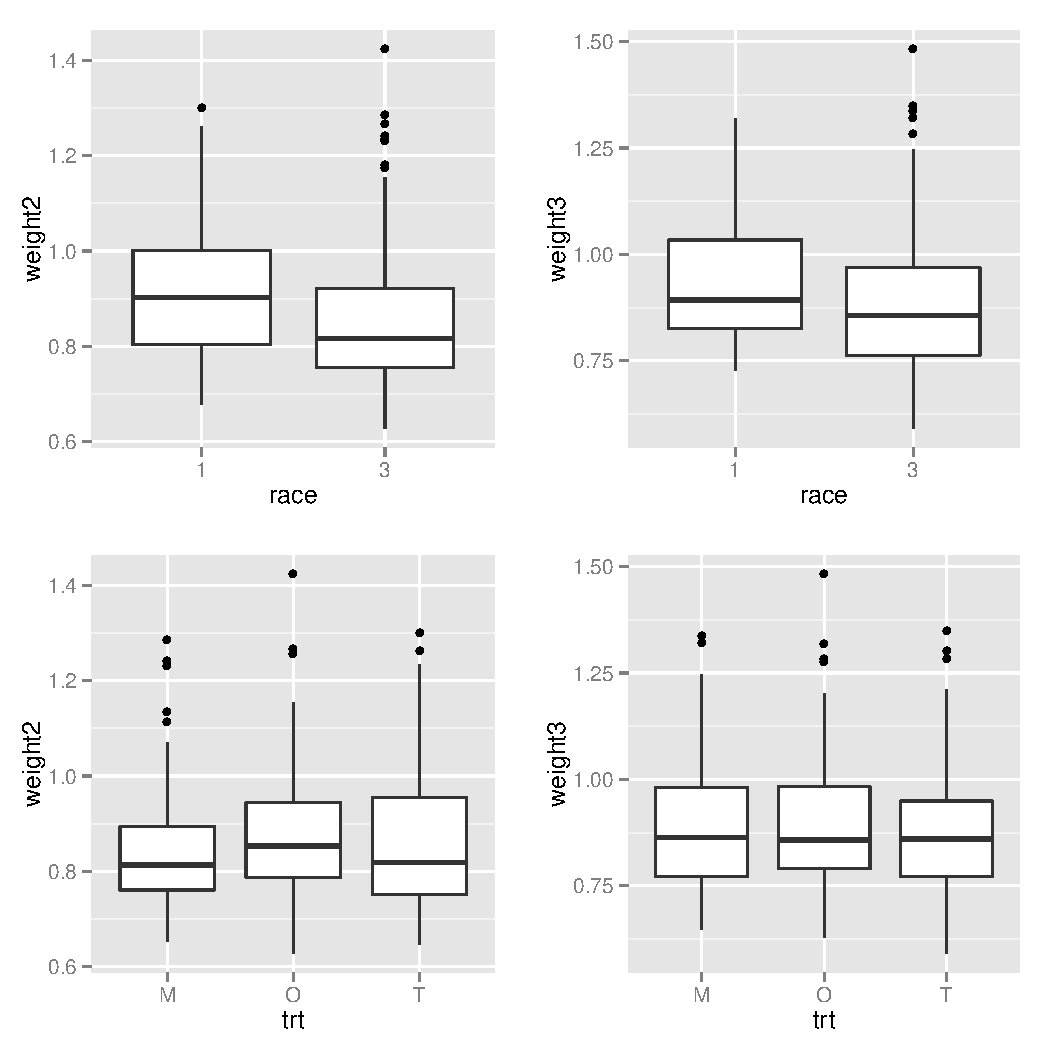
\includegraphics[scale =
    0.6]{/Users/liuminzhao/Documents/qrmissing/tours/weight-plot}}
  \caption[]{\label{fig:tours} Boxplot of weights at 6th month
    (weight2) and 18th months (weight3) vs treatments (M, O, T) and
    race (black:1, white:3)}
\end{figure}

Quantile regression models were fitted for responses \textit{weight2}
and \textit{weight3} together ($\bm Y_i = (Y_{i1}, Y_{i2})$) for
quantiles (10\%, 30\%, 50\%, 70\%, 90\%). Covariates are treatments
and races, and we assume their effects are additive. Treatment M and
Race 1 are baseline references. We fit 1,000 bootstraps to obtain the
95\% confidence intervals.

Estimates are presented in table \ref{tab:w2}. For \textit{weight2},
quantile estimates show there is no significant difference for three
treatment group through all the quantiles, because all 95 \%
confidence intervals include 0. However, when comparing weights from
two races, weights at 6th month from race 3 are generally lower than
ones from race 1. Estimates of race 3 effect to weights quantiles 10\%
up to 70\% are all significantly away from zero (negative). However,
for top weights of two races (90\% quantile), the difference is not
significant.

\begin{table}[ht]
  \renewcommand{\arraystretch}{1.3}
  \begin{center}
    \caption{Marginal quantile regression coefficients for
      Weight2}\label{tab:w2}
    \vspace{10pt}
    \begin{tabular}{rrrrr}
      \toprule
      & Intercept         & Trt.O                & Trt.T                & Race.3                \\ 
      \hline
      Weight2      &                   &                      &                      &                       \\ 
      $\tau$ = 0.1 & 0.80 (0.70, 0.86) & 0.01  ( -0.04, 0.07) & -0.01 ( -0.06, 0.06) & -0.13 ( -0.19, -0.04) \\ 
      $\tau$ = 0.3 & 0.83 (0.79, 0.92) & 0.04  ( -0.02, 0.07) & 0.02  ( -0.04, 0.05) & -0.07 ( -0.16, -0.03) \\ 
      $\tau$ = 0.5 & 0.85 (0.82, 0.98) & 0.05  ( -0.03, 0.09) & 0.04  ( -0.06, 0.07) & -0.03 ( -0.14, 0.00 ) \\ 
      $\tau$ = 0.7 & 0.95 (0.89, 1.03) & 0.03  ( -0.02, 0.10) & 0.02  ( -0.04, 0.08) & -0.04 ( -0.12, 0.00 ) \\ 
      $\tau$ = 0.9 & 0.98 (0.94, 1.11) & 0.07  ( -0.02, 0.14) & 0.06  ( -0.02, 0.14) & -0.01 ( -0.10, 0.05 ) \\
      Weight3      &                   &                      &                      &                       \\ 
      $\tau$ = 0.1 & 0.78 (0.38, 0.84) & -0.01 ( -0.07, 0.06) & -0.04 ( -0.10, 0.04) & -0.13 ( -0.18, -0.02) \\ 
      $\tau$ = 0.3 & 0.82 (0.78, 0.93) & 0.01  ( -0.04, 0.06) & -0.01 ( -0.07, 0.05) & -0.06 ( -0.16, -0.01) \\ 
      $\tau$ = 0.5 & 0.88 (0.84, 1.00) & 0.02  ( -0.06, 0.06) & 0.02  ( -0.08, 0.06) & -0.03 ( -0.13, 0.02 ) \\ 
      $\tau$ = 0.7 & 0.99 (0.92, 1.07) & 0.00  ( -0.05, 0.08) & -0.00 ( -0.07, 0.06) & -0.04 ( -0.12, 0.01 ) \\ 
      $\tau$ = 0.9 & 1.02 (0.98, 1.16) & 0.05  ( -0.06, 0.11) & 0.04  ( -0.05, 0.12) & 0.00  ( -0.10, 0.06 ) \\ 
      \bottomrule
    \end{tabular}
  \end{center}
\end{table}

For weights at 18th month (weight3), we have similar
conclusions. Confidence intervals of treatment effects on weight3 for
all quantiles (10\% up to 90\%) include zero. But after 18 months,
weights of patients from race 3 are significantly lower than ones from
race 1 only for lower quantiles (10\% to 30\%). They are not
significantly different for quantiles (50\% to 90\%).

\section{Discussion}
\label{sec:discussion}

In this paper, we have developed a marginal quantile regression model
for data with monotone dropout missingness. We use a pattern mixture
model to explain the missing mechanism. Here marginal quantile
regression coefficients are of interest instead of coefficients
conditional on random effects as in \citep{yuan2010}. In addition, our
approach allows non-parallel quantile lines over different quantiles
via modeling the mixture distribution and heterogeneity of variance.

Our method allows the missingness to be MNAR.  We illustrated how to
put informative priors for Bayesian inference and how to find
sensitivity parameters allow different missing data mechanisms .  The
recursive integration algorithm simplifies computation and can be
easily implemented even in high dimension.  Simulation study
demonstrates that our approach has smaller MSE than the traditional
frequentist method and it allows for MAR and MNAR missingness.

Our model assumes a multivariate normal distribution for each
component in the pattern mixture model, which might be too
restrictive. It is possible to replace them with a semi-parametric
model, for example, the Dirichlet process or \polya{} tree.  It would
also be interesting to assume that mixture probabilities depend on
covariates. Our future work will also include proposing a goodness of
fit test to check the model fit.

\section{Acknowledgments}


\bibliographystyle{plainnat}
% \bibliographystyle{abbrev}
\bibliography{qr-missing-reference}



\appendix 
\section{Identifiability}
\label{sec:iden}
First consider univariate case with two patterns. Suppose $y$ is
univariate and there are two patterns $R = 1$ and $R = 0$.

Before going forward to quantile regression, first we consider
identifiability problem in mean regression.

Consider a pattern mixture model:
\begin{align*}
  y | R = 1 & \sim N(\Delta + R_1 , \sigma_1) \\
  y | R = 0 & \sim N(\Delta + R_0, \sigma_0) \\
  \prob (R = 1) & = \pi \\
  E (y ) & = \theta
\end{align*}
Thus by iterated expectation, we have
\begin{align*}
  \theta = \Delta + R_1\pi + R_0(1-\pi) \\
  \Delta = \theta - \pi R_1 - (1 - \pi)R_0
\end{align*}
We can see $\Delta$ is deterministic by $\theta, R_1, R_0$. If plugged
in likelihood, we have
\begin{align*}
  y | R = 1 & \sim N(\theta + (1 - \pi)R_1 - (1 - \pi)R_0, \sigma_1) \\
  y | R = 0 & \sim N(\theta - \pi R_1 + \pi R_0, \sigma_0)
\end{align*}
Denote $\xi_1 = (\theta , R_1, R_0)$, and if $\xi_2 = (\theta, R_1+ 1,
R_0+1)$, both parameters lead to the same distribution of $\pr(y, R) =
\pr(y|R)\pr(R)$. Therefore, $\xi$ is not identifiable.  If we put
constraints on $R_1$ and $R_0$, for example $R_0 = -R_1$, then
\begin{align*}
  y | R = 1 & \sim N(\theta + 2(1 - \pi)R_1 , \sigma_1) \\
  y | R = 0 & \sim N(\theta - 2\pi R_1 , \sigma_0)
\end{align*}
thus it is identifiable. If $\xi_2 \neq \xi_1$ , then $\pr_2(y, R)
\neq \pr_1(y, R)$.

Secondly, we consider quantile regression for pattern mixture model:
\begin{align*}
  y | R = 1 & \sim N(\Delta + R_1 , \sigma_1) \\
  y | R = 0 & \sim N(\Delta + R_0, \sigma_0) \\
  \prob (R = 1) & = \pi \\
  \pr (y \leq \theta ) & = \tau
\end{align*}
where $\theta$ is the quantile estimate of interest and we does not
include covariates so far. We will show $\bm \xi = (\theta, R_1, R_0)
$ is not identifiable.

Again by iterated expectation, we have
\begin{align*}
  \tau = \pi \Phi \left( \frac{\theta - \Delta - R_1}{\sigma_1}
  \right) + (1 - \pi) \Phi \left( \frac{\theta - \Delta -
      R_0}{\sigma_0} \right)
\end{align*}
thus $\Delta$ is again deterministic by other parameters:
\begin{align*}
  \Delta = h(\theta, R_1, R_0, \sigma_1, \sigma_0 , \pi, \tau)
\end{align*}
To show $\bm \xi = (\theta, R_1, R_0, \sigma_1, \sigma_0)$ is not
identifiable, we need to find $\bm \xi^{'} \neq \bm \xi$, such that
$\pr(y|R) = \pr^{'}(y|R)$. If the last equation holds, then we must
have $\sigma_1^{'} = \sigma_1, \sigma_0^{'} = \sigma_0$, thus we still
need to find $\theta^{'} , R_1^{'}, R_0^{'}$ such that
\begin{align*}
  h(\bm \xi) + R_1 & = h(\bm \xi^{'}) + R_1^{'} \\
  h(\bm \xi) + R_0 & = h(\bm \xi^{'}) + R_0^{'}
\end{align*}
By substracting previous equations, we have $R_1^{'}- R_0^{'} = R_1-
R_0$, thus denote $R_1^{'} = R_1 + \delta$ and $R_0^{'} = R_0 +
\delta$, and let $\theta^{'} = \theta$ such that
\begin{align*}
  \Delta^{'} = h(\theta^{'}, R_1, R_0, \sigma_1, \sigma_0, \delta) =
  h(\bm \xi) - \delta = \Delta - \delta
\end{align*}
then the new parameter $\bm \xi^{'}$ yields the same distribution with
one from $\bm \xi$. Therefore $\bm \xi$ is not identifiable.

Instead, if we put constraint, for example $R_1 = -R_0$, then by
calculation, $\pr(y|R;\bm \xi) = \pr(y|R; \bm \xi^{'})$ yields $\bm
\xi = \bm \xi^{'}$.

Now consider the case with covariates. Suppose the model is
\begin{align*}
  y | R = 1, x & \sim N(\Delta + R_1 + \beta_{x1} x , \sigma_1) \\
  y | R = 0, x & \sim N(\Delta - R_1 + \beta_{x0} x, \sigma_0) \\
  \prob (R = 1) & = \pi \\
  \pr (y \leq \gamma_0 + \gamma_1 x ) & = \tau
\end{align*}
Still $\Delta$ can be determined by
\begin{align*}
  \Delta = h(x, \gamma_0, \gamma_1, R_1, \beta_{x1}, \beta_{x0},
  \sigma_1, \sigma_0, \pi , \tau)
\end{align*}
We want to show parameter $\bm \xi = (\gamma_0, \gamma_1, R_1,
\beta_{x1}, \beta_{x0}, \sigma_1, \sigma_0, \pi )$ is not identifiable
by finding $\bm \xi^{'} \neq \bm \xi$, but $\pr (y | R; \bm \xi) = \pr
(y | R; \bm \xi^{'})$. Still if the last equation holds, first we have
$\sigma_1^{'} = \sigma_1, \sigma_0^{'} = \sigma_0$, then to equate the
two means, we have
\begin{align*}
  \Delta + R_1 + \beta_{x1} x & = \Delta^{'} + R_1^{'} + \beta_{x1}^{'}x \\
  \Delta - R_1 + \beta_{x0} x & = \Delta^{'} - R_1^{'} +
  \beta_{x0}^{'}x
\end{align*}
By substracting the two equations, we have
\begin{align*}
  2R_1 + (\beta_{x1} - \beta_{x0}) x = 2R_1^{'} + (\beta_{x1}^{'} -
  \beta_{x0}^{'}) x
\end{align*}
which holds for all $x$. Thus $R_1 = R_1^{'}$ and $(\beta_{x1} -
\beta_{x0}) = (\beta_{x1}^{'} - \beta_{x0}^{'})$. Then let
\begin{align*}
  \beta_{x1}^{'} =  \beta_{x1} + \delta\\
  \beta_{x0}^{'} = \beta_{x0} + \delta
\end{align*}
and all the other parameters in $\bm \xi^{'}$ keep the same, we can
still have the same distribution of $y|R; \bm \xi$ but with different
$\bm \xi$. Therefore, $\bm \xi$ is not identifiable, especially for
$\beta_{x1} $ and $\beta_{x0}$. One solution is to restrict
$\beta_{x1} = - \beta_{x0}$ to make all the parameters identifiable.

Now consider the bivariate $(y_1, y_2)$ case, and we focus on the
identifiability issue especially on $y_2|y_1$. Suppose the model is
\begin{align*}
  y_2 | y_1, x, R = 1 \sim N(\Delta + R_1 + x\beta_{x1} + \beta_{11}y_1, \sigma_1) \\
  y_2 | y_1, x, R = 0 \sim N(\Delta - R_1 - x\beta_{x1} +
  \beta_{10}y_1, \sigma_0)
\end{align*}
Here $R$ stands for two different patterns, and missingness is not
considered.

we are wondering if $\beta_{11}$ and $\beta_{10}$ are identifiable,
say if there exists $\beta_{11}^{'}$ and $\beta_{10}^{'}$, such that
\begin{align*}
  \Delta + R_1 + x\beta_x + \beta_{11}y_1 = \Delta^{'} + R_1^{'} + x\beta_{x}^{'} + \beta_{11}^{'}y_1\\
  \Delta - R_1 - x\beta_x + \beta_{10}y_1 = \Delta^{'} - R_1^{'} -
  x\beta_{x}^{'} + \beta_{10}^{'}y_1
\end{align*} 
still by substracting two equations, we have $R_1 = R_1^{'}$ and
$\beta_x = \beta_x^{'}$. Considering $\Delta$ is determined by
integrating out $y_1$, such that matching the two sides of the above
equation for coefficient of $y_1$, we must have $\beta_{11} =
\beta_{11}^{'}$ and $\beta_{10} = \beta_{10}^{'}$, therefore, $\bm
\xi$ is identifiable.

For identifiability issue in heterogeneous model described in section
[ref], it is easy to show there is no trouble with heterogeneity
parameters $\alpha$, analog to the linear model case. For the other
parameters, it can be found similar to the above discussion.

\section{Proof of Lemma \ref{sec:lemma}}
\label{sec:proof}
\begin{itemize}
\item Denote
  \begin{displaymath}
    I(a,b) = \int \Phi \left( \frac{x-b}{a} \right)\phi(x) dx ,
  \end{displaymath}
  where $\Phi$ is the standard normal cdf and $\phi$ is the standard
  normal pdf and $a > 0$.
  \begin{align*}
    \frac{\partial I(a,b)}{\partial b} & = - \frac{1}{a} \int \phi \left( \frac{x-b}{a} \right) \phi(x) dx \\
    & = - \frac{1}{\sqrt{2 \pi} \sqrt{a^2+1}} \exp \left( - \frac{b^2}{2(a^2+1)} \right)\\
    & = -\frac{1}{\sqrt{a^2+1}} \phi \left( \frac{b}{\sqrt{a^2+1}}
    \right).
  \end{align*}
  Since $I(a, \infty) = 0$,
  \begin{align}
    I(a,b) &= - \frac{1}{\sqrt{a^2+1}} \int_b^{\infty} \phi \left( \frac{s}{\sqrt{a^2+1}} \right) ds \nonumber \\
    &= \int_{b/\sqrt{a^2+1}}^{\infty} \phi(t) dt \nonumber\\
    \label{eq:int}
    & = 1- \Phi(b/\sqrt{a^2+1}).
  \end{align}
  For $a < 0$,
  \begin{align*}
    \frac{\partial I(a,b)}{\partial b} & = - \frac{1}{a} \int \phi \left( \frac{x-b}{a} \right) \phi(x) dx \\
    & = - \frac{sgn(a)}{\sqrt{2 \pi} \sqrt{a^2+1}} \exp \left( - \frac{b^2}{2(a^2+1)} \right)\\
    & = -\frac{sgn(a)}{\sqrt{a^2+1}} \phi \left(
      \frac{b}{\sqrt{a^2+1}} \right).
  \end{align*}
  Since $I(a, -\infty) = 0$:
  \begin{align}
    I(a,b) &= \int^{b/\sqrt{a^2+1}}_{-\infty} \phi(t) dt \nonumber\\
    \label{eq:intneg}
    & = \Phi(b/\sqrt{a^2+1}).
  \end{align}
\item For integrating over a normal distribution with mean $\mu$ and
  standard deviation $\sigma$:
  \begin{align*}
    \int \Phi(x)d\Phi(x; \mu, \sigma) & = \int \Phi(x) \frac{1}{\sigma} \phi \left( \frac{x-\mu}{\sigma} \right) dx \\
    & = \int \Phi(\sigma t + \mu)\phi(t) dt \\
    & = 1 - \Phi(-\mu/\sigma/\sqrt{1/\sigma^2+1}).
  \end{align*}
  The last equation holds by (\ref{eq:int})
\item For integrating a $\textrm{N}(b, a)$ CDF over another normal
  distribution ($\textrm{N}(\mu, \sigma$)):
  \begin{align}
    \int \Phi \left( \frac{x-b}{a} \right) d\Phi(x; \mu, \sigma) & = \int \Phi \left( \frac{x-b}{a} \right) \frac{1}{\sigma} \phi \left( \frac{x-\mu}{\sigma} \right) dx \nonumber\\
    &= \int \Phi \left( \frac{\sigma y + \mu - b}{a}  \right) \phi(y) dy \nonumber \\
    \label{eq:intg1}
    & = 1- \Phi \left( \frac{b-\mu}{\sigma} /
      \sqrt{\frac{a^2}{\sigma^2}+1} \right).
  \end{align}
  If $a < 0$,
  \begin{equation}
    \label{eq:intg2}
    \int \Phi \left( \frac{x-b}{a} \right) d\Phi(x; \mu, \sigma) = \Phi \left( \frac{b-\mu}{\sigma} / \sqrt{\frac{a^2}{\sigma^2}+1} \right).
  \end{equation}

\end{itemize}

\section{Maximum Likelihood Estimation Using Adaptive Gradient Descent
  Algorithm}
\label{sec:agda}

See section \ref{sec:mle} for notations.

The likelihood can be maximized via the following algorithms:
\begin{enumerate}
\item Initialize $\bm \xi$
\item \label{item:der} calculate $\partial J(\bm \xi) / \partial
  \xi_j$ for all $j$,
\item update $\bm \xi$ by adaptive gradient descent algorithm
  described in \citep{ried1993} for all $j$
\item evaluate new $J(\bm \xi)$
\item if the amount of descent of $J ( \bm \xi)$ is great than certain
  number, say $10^{-3}$, then go back to step \ref{item:der} and
  repeat. Otherwise, algorithm converges.
\end{enumerate}

We can use numerical approximation to calculate $\partial J(\bm
\xi)/\partial \xi_j$ in algorithm step \ref{item:der}. For example,
when $j = 1$,
\begin{displaymath}
  \frac{\partial J(\bm \xi)}{\partial \xi_1} \approx \frac{J(\xi_1 + \epsilon, \xi_2, \ldots) - J(\xi_1 - \epsilon, \xi_2 , \ldots)}{2\epsilon}.
\end{displaymath}

\end{document}

%%% Local Variables: 
%%% mode: latex
%%% TeX-master: t
%%% End: 
